\section{Music Structure Analysis as downstream task}

While the usefulness of deep audio embeddings can be evaluated in several scenarios, we have chosen a core MIR task for its popularity and complexity: Music Structure Analysis (MSA). This interdisciplinary field aims to understand the structure of music \cite{Nieto2020Audio-BasedApplications}. However, due to subjectivity, ambiguity, and data scarcity, audio-based MSA faces challenges like boundary placement ambiguity and similarity quantification \cite{NietoPerceptualMusic}. 

The main principles of MSA were initially defined as homogeneity, novelty, and repetition, with the addition of regularity. 

\subsection{SALAMI dataset}

SALAMI (Structural Analysis of Large Amounts of Music Information) \cite{Smith2011DESIGNANNOTATIONS} aims to conduct massive structural analyses of different types of music. The project covers diverse music, from Western pop to Indian classical and from live to studio recordings.

\subsubsection{Formal analysis definition and approaches}
Formal analysis, in this context, doesn't refer to classifying the piece into a formal type (e.g., sonata, song, or canon) or reducing it into its Ursatz as in Schenkerian analysis. Instead, it means organizing and dividing the piece into specific sections and understanding how they relate.

The proposed method integrates aspects of three approaches: perceptual, functional, and transcription, enabling a comprehensive analysis of a wide range of music pieces using a limited vocabulary. 

It considers the hierarchical nature of music structure and employs markers to partially address the challenge of determining the appropriate timescale for analysis. 

The perceptual approach involves segmenting and labeling sections based on harmonic or rhythmic boundaries, although it may not accurately reflect the structural roles of similar-sounding sections. 

The functional approach categorizes the song into components like verses and choruses, potentially leading to varied labels for identical music or identical labels for different musical ideas based on their function. 

The transcription approach records musical parameters directly, such as chord patterns and instrumentation, providing a less subjective method, but it might not capture the complete structure of the piece.

\section{\textit{Embeddiogram} feature}

The Embeddiogram is derived by applying a pre-trained neural network model to windowed segments of an audio signal, generating a sequence of embedding vectors. These embedding vectors collectively form a high-dimensional description of the audio signal's structure and content.

Below is a detailed explanation of computing the Embeddiogram from a given audio signal. This process comprises five key steps, including loading the audio data, slicing the audio data into windowed segments, processing each window using a pre-trained model to produce an embedding, collecting these embeddings, and finally normalizing the Embeddiogram. 

\begin{enumerate}
\item \textbf{Load the audio data}: The audio data is loaded into memory as a one-dimensional array of length $N$.

\item \textbf{Slice the audio data}: The audio data is segmented into overlapping windows. Each window contains $w$ samples, and consecutive windows are separated by $h$. This gives a total of $H$ windows, defined as:
\begin{equation}
H = 1 + \left\lfloor \frac{N - w}{h} \right\rfloor
\end{equation}
In the case where $\left( N - w \right) \mod h > 0$, we have $H += 1$ to account for the final, potentially smaller, window.

\item \textbf{Process each window}: Each window of audio data is processed independently, passed through the pre-trained neural network model and transformed into an embedding vector. Formally, for each window $w_i$ of audio data, we have:
\begin{equation}
\text{embedding}_i = \text{model}(w_i)
\end{equation}

\item \textbf{Collect the embeddings}: The embedding vectors are collected and stacked together. Each row represents a feature vector for a given time frame to form the \textit{Embeddiogram}, denoted as $\text{embeddiogram}$:
\begin{equation}
\text{embeddiogram} = \begin{bmatrix} \text{embedding}_1 \\ \text{embedding}_2 \\ \vdots \\ \text{embedding}_H \end{bmatrix}
\end{equation}

\item \textbf{Normalize the Embeddiogram}: The Embeddiogram is normalized to have a minimum value of 0 and a maximum value of 1. The normalization process is given by:
\begin{equation}
E'_{ij} = \frac{e_{ij} - \min(E)}{\max(E) - \min(E)}
\end{equation}
\end{enumerate}

%\begin{figure}
    %\centering
    %\includegraphics[width=\textwidth]{figures/images/embeddiogram SALAMI 3.png}
    %\caption[Embeddiogram]{Embeddiogram computed from...}
    %\label{fig:embeddiogram}
%\end{figure}


%\begin{figure}
    %\centering
    %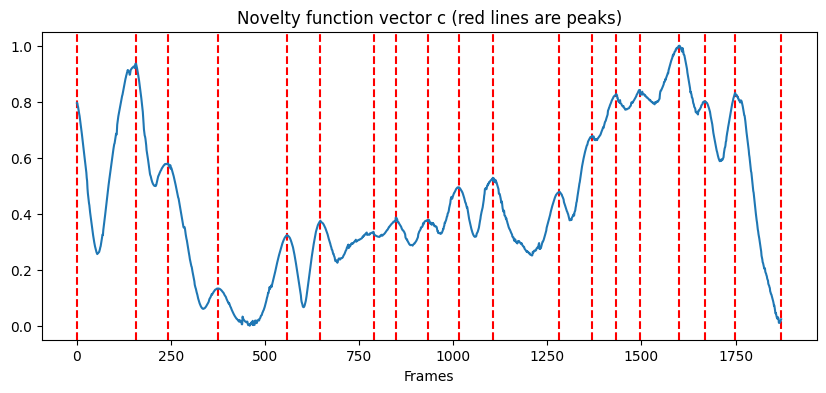
\includegraphics[width=\textwidth]{figures/images/noveltypeaks_SALAMI_track_2.png}
    %\caption[Novelty curve]{Caption}
    %\label{fig:embeddiogram}
%\end{figure}

\begin{figure}[ht]
    \centering
    \begin{minipage}{0.45\textwidth}
        \centering
        \includegraphics[width=0.9\textwidth]{figures/images/recurrence plot SALAMI 3.png} % first figure itself
        \caption{first figure}
    \end{minipage}\hfill
    \begin{minipage}{0.45\textwidth}
        \centering
        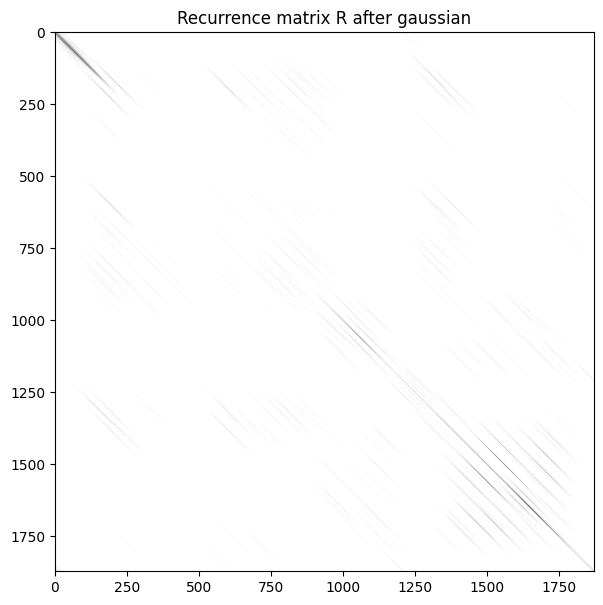
\includegraphics[width=0.9\textwidth]{figures/images/Rec_matrix_smooth_SALAMI_track_2.png} % second figure itself
        \caption{second figure}
    \end{minipage}
\end{figure}

